\section{A visual design space for DOI analysis}

The previous sections illustrated the difference between AOI and DOI data and the range of DOI tasks, providing an intuition that existing AOI methods do not directly extend to DOI data. First, AOI visualizations such as scanpaths and scarfplots cannot handle the scale of DOI data, which is granular and captured over long experiments. Second, AOI visualizations cannot show or leverage the many attributes that can describe a typical DOI.  Third, collecting visual interest in richly annotated DOIs, over long experiments, from many users, can support analyses different than those typical of AOI data. This section explores a design space of visual solutions that can alleviate these shortcomings.

\begin{figure}[!htb]
  \centering
	%\includegraphics[width=\linewidth]{images/Scanpaths.png}
  \includegraphics[width=\linewidth]{images/Scanpaths.eps}
  \caption{Scanpaths of real DOI data. (left) Data is shown separately for each user. Depicted DOIs are the same for all four users, enabling the comparison of the scanpath profile; the top two users viewed simialr data. (right) Users' data are shown next to each other for each DOI; we notice that the four users cluster into two pairs, based on their interests.}
	\label{fig:scanpath}
\end{figure}

Thus, DOI visualizations should allow analysts to explore DOI data at many levels of detail, including multiple temporal scales (e.g., seconds vs. minutes) and data granularities (e.g., individual vs. categories of DOIs).  DOI attributes should be shown visually and queried flexibly to allow analysts to detect correlations between a user's interest in data and that data's properties. Attributes should be used to deal with the scale of the data by allowing users to filter, highlight, and aggregate data with specific attribute values. Finally, visualizations need to support the DOI task taxonomy. 

Next, we analyze the design space for visual DOI analysis in more detail. Given the scale DOI data and the breadth of DOI tasks, visual encodings should be augmented with interaction capabilities. To ensure that our discussion captures all visual design dimensions, we ground it in Yi's taxonomy of interaction tasks~\cite{yi2007toward}, which includes seven categories of visual operations: Encoding, Selection, Reconfiguration, Exploration, Abstraction/Elaboration, Filtering, and Connection/Comparison~\cite{yi2007toward}. We will discuss novel visual solutions by starting from existing AOI visualizations and describing how they may be extended and redesigned to support DOI requirements. 


\begin{figure*}
  \centering
	%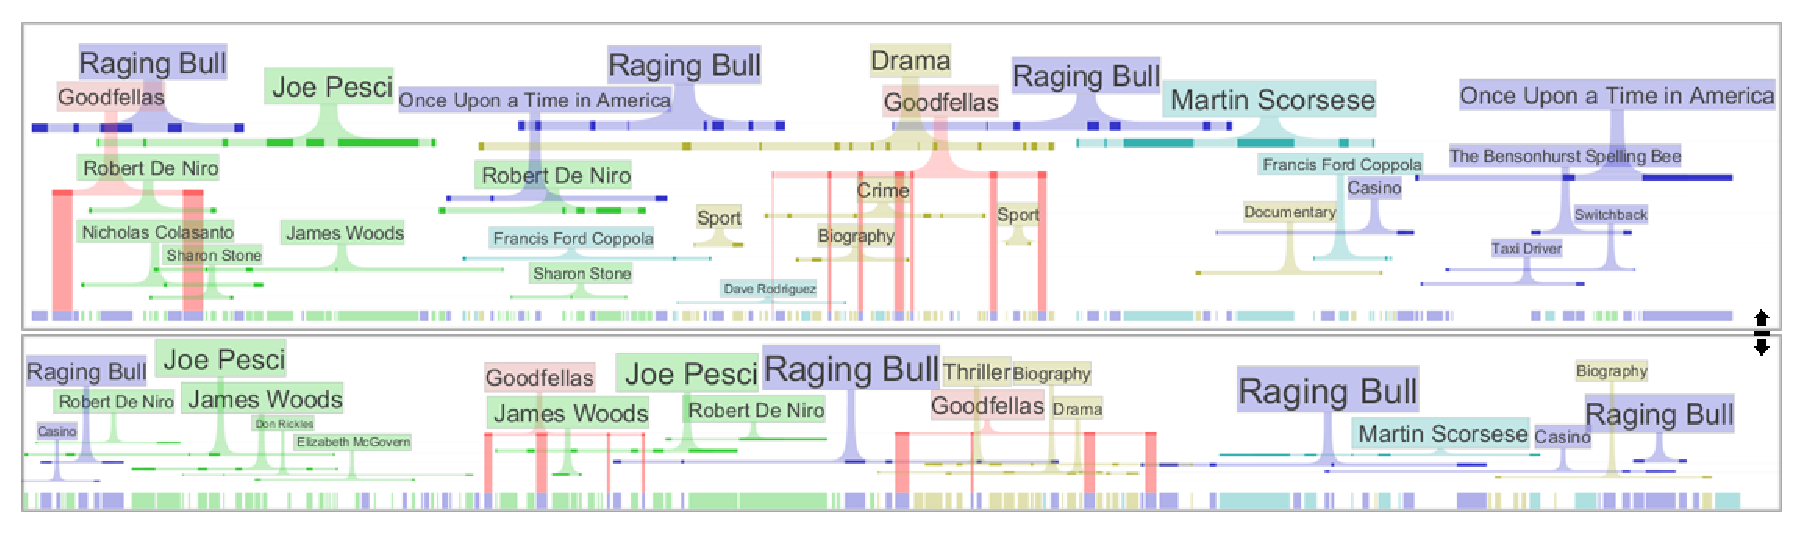
\includegraphics[width=0.95\linewidth]{images/Scarfs.eps}
  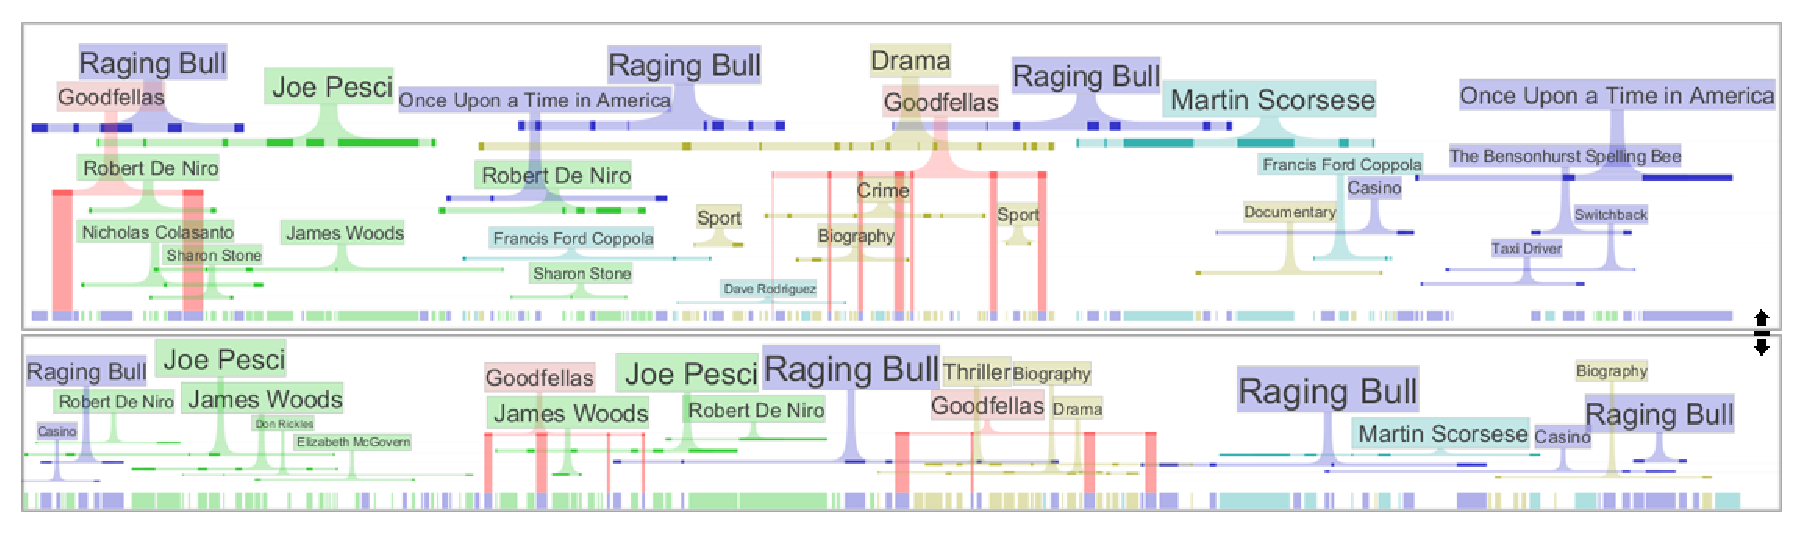
\includegraphics[width=0.95\linewidth]{images/Scarfs.eps}
  \caption{Re-imagined scarfplots for movie DOI data, sketched for two users. DOI are labeled explicitly, and scaled according to how much they were viewed around particular time-points. Resizing a users' plot vertically would show less or more data. A selection for one user (Goodfellas) is highlighted in all data. }
	\label{fig:scarfs}
\end{figure*}

\subsection{Encoding}
\label{sec:Encoding}
Encoding determines how data should be shown visually~\cite{yi2007toward}. Encoding design options and requirements of DOI visualizations are detailed below.

\noindent \textbf{Show many DOIs :} AOI visualizations such as scarfplots identify specific AOIs via distinctive colors. This method does not scale to many DOIs, and methods that identify DOIs explicitly (e.g., through a label), such as scan-paths or transition matrices, are likely preferable. 

Also, showing all DOIs viewed in an experiment is not always possible, especially when viewing data from many users. For example, a scanpath of ten users, each having viewed $100$ DOIs would have a thousand rows and be cluttered. One solution is to show only the most viewed DOIs, as done for visualizations shown in Figures~\ref{fig:scanpath},~\ref{fig:scarfs},~\ref{fig:heatmap},~\ref{fig:matrixGraph}, and to alot DOI space that is proportional to how often they are viewed, as exemplified in Figure~\ref{fig:heatmap}. This prioritization approach is likely appropriate as Alam et al. showed that even though users view many DOIs during an extended analysis, they focus most of their attention on a smaller subset of them. 

Finally, DOI attributes make it possible to collapse multiple DOIs into categories to reduce the amount of information shown, as discussed in section~\ref{sec:Interaction}, Abstract/Elaborate.

\noindent \textbf{Showing long experiments} can be supported by exploring data at multiple time scales, and relies on the ability of visualizations to aggregate data over times longer than a single fixation. Such encodings are difficult to imagine for scanpaths and scarfplots, as they depict direct transitions between objects at each of a user's fixations, a problem also for showing multiple DOIs viewed within a single fixation. Alternatively, heatmaps (Figure~\ref{fig:heatmap}) and AOI/DOI-rivers can show multiple DOIs within a single time-frame. We discuss temporal scales in more detail in section~\ref{sec:Interaction}, Abstract/Elaborate. A second way to deal with data collected during long experiments is to restrict views to time windows using filtering interactions, as discussed in section~\ref{sec:Interaction}, Filtering.

\begin{figure}[htb]
  \centering
  %\includegraphics[width=0.9\linewidth]{images/Heatmap.PNG}
	\includegraphics[width=0.9\linewidth]{images/Heatmap.eps}
  \caption{Heatmap of real DOI data. User data is shown separately. DOI-rows are scaled vertically to make DOIs viewed often more salient. DOIs are ordered by viewing amount; those beyond a threshold are not shown.
  A time-window (white section) helps prioritize which data is shown.}
	\label{fig:heatmap}
\end{figure}


\noindent \textbf{Showing DOI attributes} can be supported via conventional techniques such as linking DOI attributes to visual channels (e.g., color, shape) or by relying on glyph designs. Displaying DOI attributes can enable analysts to visually detect how DOIs with similar properties clusters over time (time tasks 5-9). For such tasks to be possible, in addition to showing attributes, DOIs need to be grouped based on when they were viewed or in what transitions they were involved. For example, scarf-plots inherently order DOIs by time (Figure~\ref{fig:scarfs}), but scan-paths and transition matrices have to be clustered to group together co-viewed DOIs (Figure~\ref{fig:scanpath}). Additionally, showing multiple attributes for each DOI facilitates a visual approximation of attribute-derived measures, supporting summarization tasks 1-4. 

\noindent \textbf{Reducing clutter} is essential in busy DOI visualizations. Clustering is one effective way to impose order on visualizations. Figure~\ref{fig:scanpath} shows scanpaths that orders DOIs based on how often there are transitions between them. This in effect shortens the vertical transition in the paths. Second, linking DOI appearance to their attributes can divide DOIs into data categories or layers that are visually separable, in accordance with Gestalt principles. Third, reducing shown information using semantic zooming and DOI grouping, and highlighting and filtering, can also reduce clutter, as discussed in the next sections. 

\noindent \textbf{Supporting tasks :} To support transition tasks 10-14, visualizations should support variable definitions of transitions. The designs in Figure~\ref{fig:matrixGraph} show how transitions may be defined as the viewing of a DOI within a short time interval of another, rather than immediately after, and that this time interval could be variable. This is similar to $VA^2$'s recent use of wild-cards when computing AOI sequences~\cite{blascheck2016va}. Furthermore, we hypothesize that in the context of DOIs, transition graphs could reveal DOI sequences better than matrices, since node-link diagrams are superior at showing paths~\cite{ghoniem2004comparison}.

\begin{figure}[htb]
  \centering
  %\includegraphics[width=0.98\linewidth]{images/MatrixGraph.png}
	\includegraphics[width=0.98\linewidth]{images/MatrixGraph.eps}
  \caption{Transition matrix and graph of real DOI data. Both support multiple time-scales by allowing transitions to be defined flexibly, depending on the maximum time allowed to pass between when a first and second object are viewed. The graph shows often viewed objects larger.}
	\label{fig:matrixGraph}
\end{figure}

A further factor needs to be considered when supporting analyses of DOI data from many subjects. Visualization data-sets can support hundreds or thousands of DOIs, which subjects, based on their interests and exploration, will only see small subsets of. These subsets may differ significantly between subjects, leading to a tradeoff: should visualizations be optimized to best show a single user's behavior, or to show a user's behavior in the context of other users' data? The scan-paths in Figure~\ref{fig:scanpath} show DOIs that were viewed by all subjects, and use the same DOI-set and ordering for each user. Alternatively, each subjects' scan-path could also show and order DOIs based solely on that subject's data. The former approach shows less relevant data for each user but makes it easy to compare user behavior, while the latter would show more relevant data for each user but would hinder comparison. Similarly, scanpaths can be separate or integrate individual users' data as shown in Figure~\ref{fig:scanpath}, making it easier or harder to compare subjects.

\subsection{Interaction}
\label{sec:Interaction}
\noindent \textbf{Selection :} Selections allow users to track interesting objects by marking them~\cite{yi2007toward}. With respect to selection targets, DOI methods support selections of DOIs, DOI categories, users, and time intervals.  As for methods of selection, two options are possible: `in situ' selections of DOIs shown in the visualization, and query-based selections of DOIs by attribute values. Finally, selected items should be highlighted visually and brushing and linking should translate selections over multiple views, supporting connect and compare interactions. Figures~\ref{fig:scanpath},~\ref{fig:scarfs},~\ref{fig:heatmap} exemplify DOI selections, time-window selections, and brushing and linking.

\noindent \textbf{Reconfiguration :}
Reconfigurations change the spatial arrangement of data.  In section~\ref{sec:Encoding} we already discussed the benefit of clustering co-viewed DOIs to reduce clutter and to support the detection of correlations between DOI categories and when they are viewed. Additionally, DOIs should be orderable based on their attributes. Similarly, clustering and arranging subjects by their behavior can create more organized visualizations, while the ability to cluster subjects on their background or demographic data (e.g., expert vs. naive subjects) can support tasks typical of human experimentation. Finally, visualizations should also support interactive repositioning (e.g., of users, DOIs), to allow analysts to manually arrange and group items.


\noindent \textbf{Exploration} enables users to analyze different subsets of data instances. DOI data visualizations should support time-scrolling, panning, and zooming efficiently. Exploration options also include the ability to flexibly define which DOI attributes should be mapped visually, given that the number of variables that can be visually encoded concurrent may be limited. 
	
\noindent \textbf{Abstract/Elaborate} interactions allow users to control a visualization's level of abstraction. Our discussion on encoding emphasizes the need for representations that support analyses at multiple time-scales, DOI grouping, and the ability to control the amount of data shown. 

First, semantic zooming can be an efficient way to explore different time scales and involves aggregating and summarizing data over variable time-steps (e.g., milliseconds to minutes). An alternative to semantic zooming are pixel based techniques which allow individual viewing-events to merge and blend together visually\cite{keim2000designing}. The re-imagined scarfplot design in Figure~\ref{fig:scarfs} exemplifies the first approach by grouping co-viewed elements together, while the heatmap in Figure~\ref{fig:heatmap}, the second. The transition matrix Figure~\ref{fig:matrixGraph} also exemplify semantic zooming by providing the ability to interactively adjust the time-step used for defining transitions.  

Second, DOIs could be grouped by using attribute queries to define DOI categories, by exploiting DOI hierarchies (i.e., DOIs that are contained by other DOIs), or manually. Aggregating DOIs visually can again be done semantically, by allowing analysts to explicitly collapse multiple DOIs into single ones, or by showing data in a way that allows categories to emerge and separate visually. 

 Finally, details on demand can give access to additional data via tool-tips and auxiliary information data panels, populated with data obtained through brushing and linking.
  
	
\noindent \textbf{Filtering} enables users to change the set of data items being presented based on specific conditions, and should be possible on all selectable data categories previously mentioned. DOIs should be hidden or revealed based on their attributes, how often they are viewed, when they are viewed, and which users view them (e.g., ``Show only DOIs that both of two selected users viewed'').

The number of DOIs shown could be controlled directly (e.g., ``Show top $25\%$ most viewed data''), or by adjusting the amount of space allotted to users and filling it with as much data as can fit, as suggested in Figure~\ref{fig:scarfs}. The latter is a useful way of controlling the amount of information based on available screen space and how many users or time-intervals one needs to compare.

Defining time-windows of interest can support both reconfiguration and filtering interactions. Since DOI visualizations will likely need to prioritize which data to show, defining specific time windows that such configurations should be based on, can support novel tasks. For example, by prioritizing the display of data that subjects viewed late in an experiment, an analysts could un-clutter the visualization of data which subjects viewed during preliminary exploration and search processes, and more clearly reveal how final data interests crystallize.


	
\noindent \textbf{Connection/Comparison} interactions show associations and relationships between data items (tasks 15-20), and can be implemented using one of Gleicher et al.'s visual comparison methods: juxtaposition, superposition, and encoding of differences~\cite{gleicher2011visual}. To support juxtaposition, data from multiple users or from multiple time-intervals should be shown using compact, stackable, and comparable visualizations. The designs in Figures~\ref{fig:scanpath},~\ref{fig:scarfs},~\ref{fig:heatmap},~\ref{fig:matrixGraph} can be resized to show more or less of a user's data, to multiple user-views to fit in a single screen, and the scanpaths use the same DOI ordering for all users to support comparison. Superposition is exemplified in the right panel of Figure~\ref{fig:scanpath}. Selecting and highlighting overlaps and differences (e.g., ``Show DOIs viewed by all participants'', ``Show DOIs that are unique to a subject'') can implement the third method of comparison. Brushing and linking across users and across time would support all comparison and correlation tasks.

Finally, clustering can reveal similarities between users or time-intervals computationally. AOI sequences of multiple users have previously been clustered using a string-edit distance~\cite{kurzhals2014iseecube}. This gave good results for short, highly constrained perceptual tasks with few AOIs. However, this distance measure may not be robust enough to handle DOI data collected over long, open-ended tasks, since such data is not temporally-aligned and is bound to differ at the key-hole level that string-editing operates. Instead, comparing users in a space of derived features (e.g., DOIs they viewed most, common DOI transitions or sequences) may be more robust to local differences. It may also allow features to be included in and excluded from a distance measure, thus enabling an exploration of which features explain observed behavior.


